
\lstinputlisting[language=bash,basicstyle=\small]{python_codes/fieldstone_107/keywords}

\begin{center}
Code at \url{https://github.com/cedrict/fieldstone/tree/master/python_codes/fieldstone_107}
\end{center}

\par\noindent\rule{\textwidth}{0.4pt}

{\sl This stone was developed in collaboration with Zolt{\'a}n Erd{\H{o}}s}. 
\index{contributors}{Z. Erd{\H{o}}s}

\par\noindent\rule{\textwidth}{0.4pt}

%%%%%%%%%%%%%%%%%%%%%%%%%%%%%%%%%%%%%%%%%%%%%%%%%%%%%%%%%%%%%%%%%%%%%%%%%%%%%%%%%%%%%%%%%%%%%%%%%%%%



This stone is based on WAFLE, a simple finite element code which solves the mass, momentum and heat transfer 
equations in two dimensions in a porous media. This  code was written by M. Saltnes (Master student at 
the Dept. of Mathematics, University of Bergen) and myself between September 2009 and May 2010. The title 
of the thesis is "Finite Element Modelling for Buoyancy Driven Flow in Natural Geothermal Systems". 

\vspace{1cm}

We use biquadratic polynomials $(Q_2)$ for velocity and temperature, 
and bilinear polynomials ($Q_1$) for pressure.

The mass and momentum conservation equations yield the following system 

\[
\left(
\begin{array}{ccc}
\N_{xx} & \N_{xy} & \G_x \\
\N_{yx} & \N_{yy} & \G_y \\
\HH_{x} & \HH_y & 0 
\end{array}
\right)
\cdot
\left(
\begin{array}{c}
\vec{\cal V}_x \\
\vec{\cal V}_y \\ 
\vec{\cal P}
\end{array}
\right)
=
\left(
\begin{array}{c}
\vec{f}_x \\ 
\vec{f}_y \\ 
\vec{h}
\end{array}
\right)
\]
where the right hand side vectors $\vec{f}_x $ and $\vec{f}_y$ depend on temperature via the density. 

The discretised steady state heat transport equation simply is 
\[
({\K}_a + {\K}_d ) \cdot \vec{\cal T}= \vec{0}
\]
where $\K_a$ is the advection matrix (built with the previously obtained velocity) 
and $\K_d$ is the diffusion matrix.

We iterate this out using a simple relaxation technique \cite{vyrc13} as in \stone 20 and 51 for example.
After I have solved for velocity (using the most recent temperature field in the rhs), 
the velocity is relaxed as follows:
\[
\vec{\cal V}_x^k = \gamma \vec{\cal V}_x^k + (1-\gamma) \vec{\cal V}_x^{k-1}
\]
\[
\vec{\cal V}_y^k = \gamma \vec{\cal V}_y^k + (1-\gamma) \vec{\cal V}_y^{k-1}
\]
and after having solved for temperature having used the most recent velocity field, the same approach is taken for temperature:
\[
\vec{\cal T}^k = \gamma \vec{\cal T}^k + (1-\gamma) \vec{\cal T}^{k-1}
\]
where the relaxation parameter $\gamma$ is between 0 and 1.
Convergence is reached when two consecutive velocity and temperature fields
do not change anymore.

\vspace{1cm}

WARNING no periodic boundary conditions yet

WARNING average heat coeffs with solid

\Literature: Section 10 in Simpson's book \cite{simp17}

%...............................................
\subsection*{Manufactured solution}

Before we start using the code for convection experiments, we wish to benchmark it
with a manufactured solution. 
We start from the velocity of the Donea \& Huerta benchmark in the unit square:
\begin{eqnarray}
u(x,y) &=& x^2(1- x)^2 (2y - 6y^2 + 4y^3)  \\
v(x,y) &=& -y^2 (1 - y)^2 (2x - 6x^2 + 4x^3) 
\end{eqnarray}
which we know to be divergence-free.
We postulate $p(x,y)=-x^3y^3+0.0625$ (so that it is on average zero over the domain) 
and set $\rho=1$, ${\bm K}={\bm 1}$, $\eta_f=1$ so that 
\begin{eqnarray} 
g_x(x,y) 
&=& -u(x,y) - \partial_x p \nn\\
&=& -u(x,y) +3x^2y^3 \nn\\ 
g_y(x,y)  
&=& -v(x,y) - \partial_y p \nn\\ 
&=& -v(x,y) +3x^3y^2 \nn
\end{eqnarray}

\begin{center}
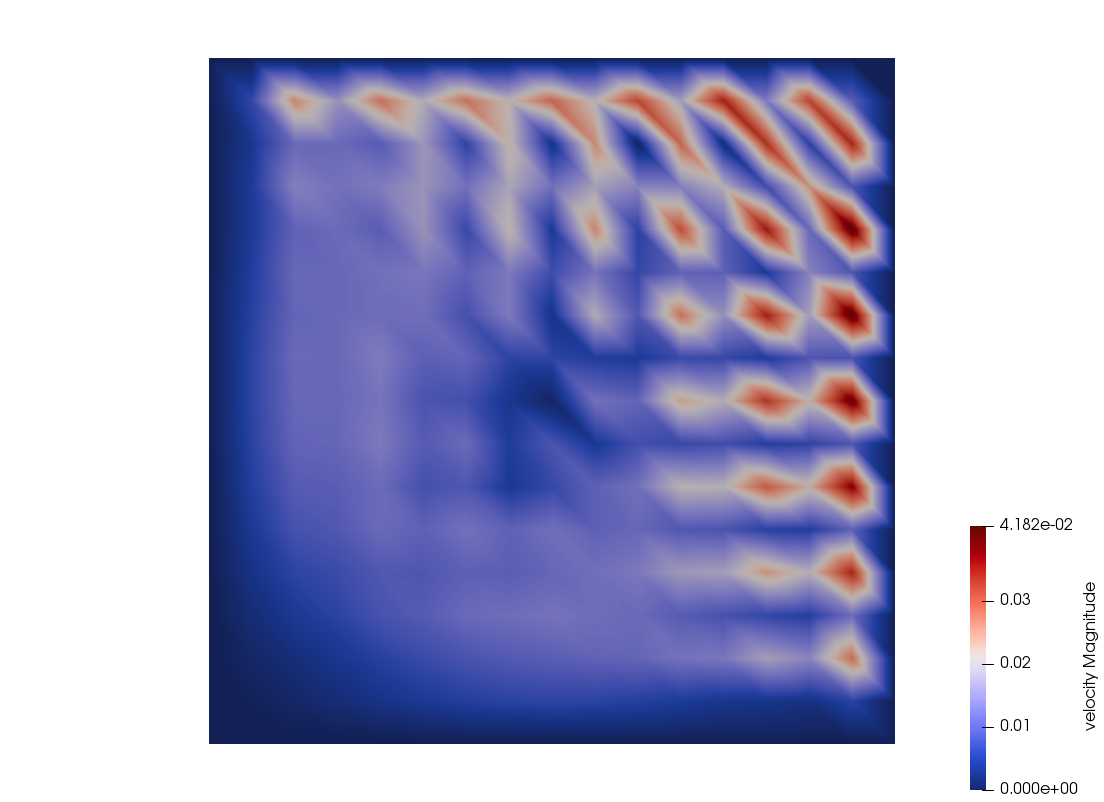
\includegraphics[width=3cm]{python_codes/fieldstone_107/results/mms/q2q1/vel08}
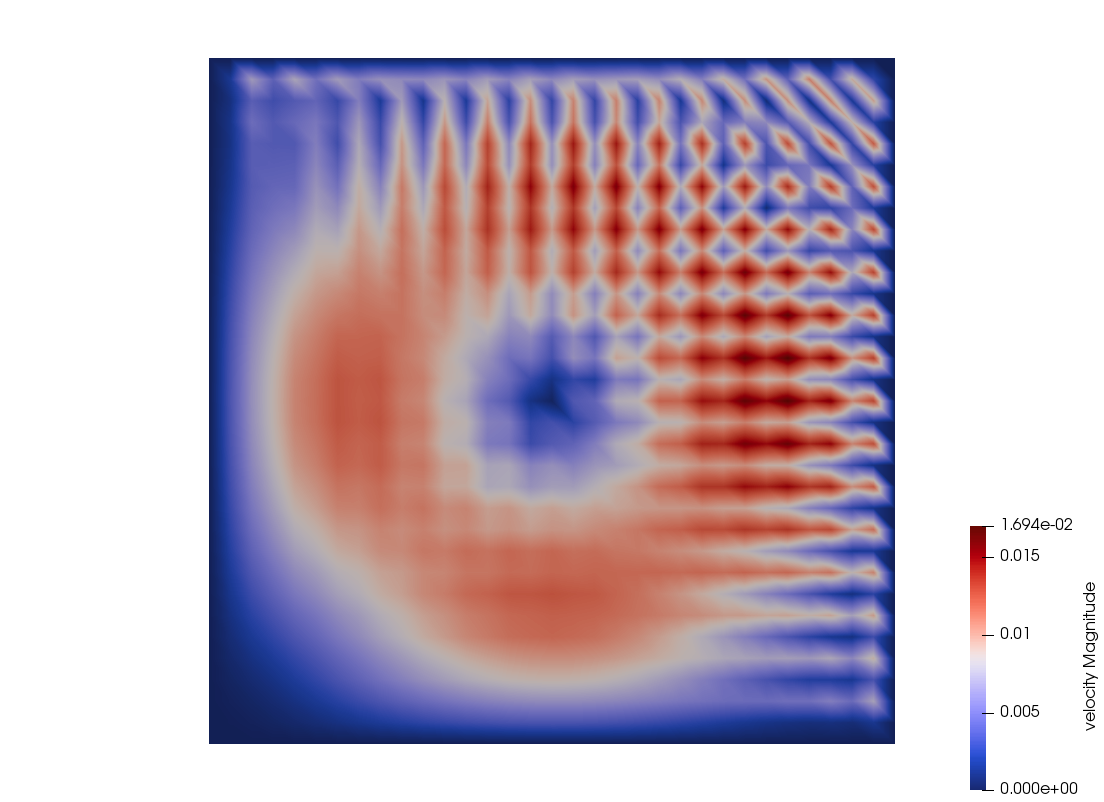
\includegraphics[width=3cm]{python_codes/fieldstone_107/results/mms/q2q1/vel16}
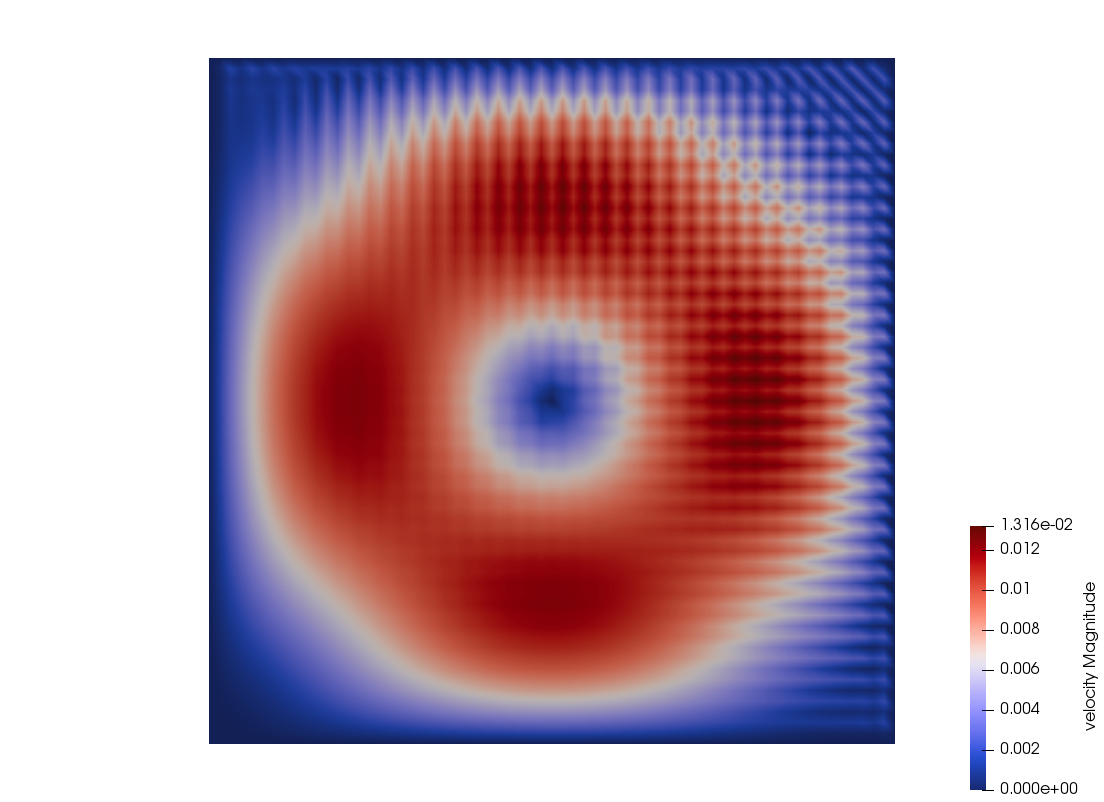
\includegraphics[width=3cm]{python_codes/fieldstone_107/results/mms/q2q1/vel32}
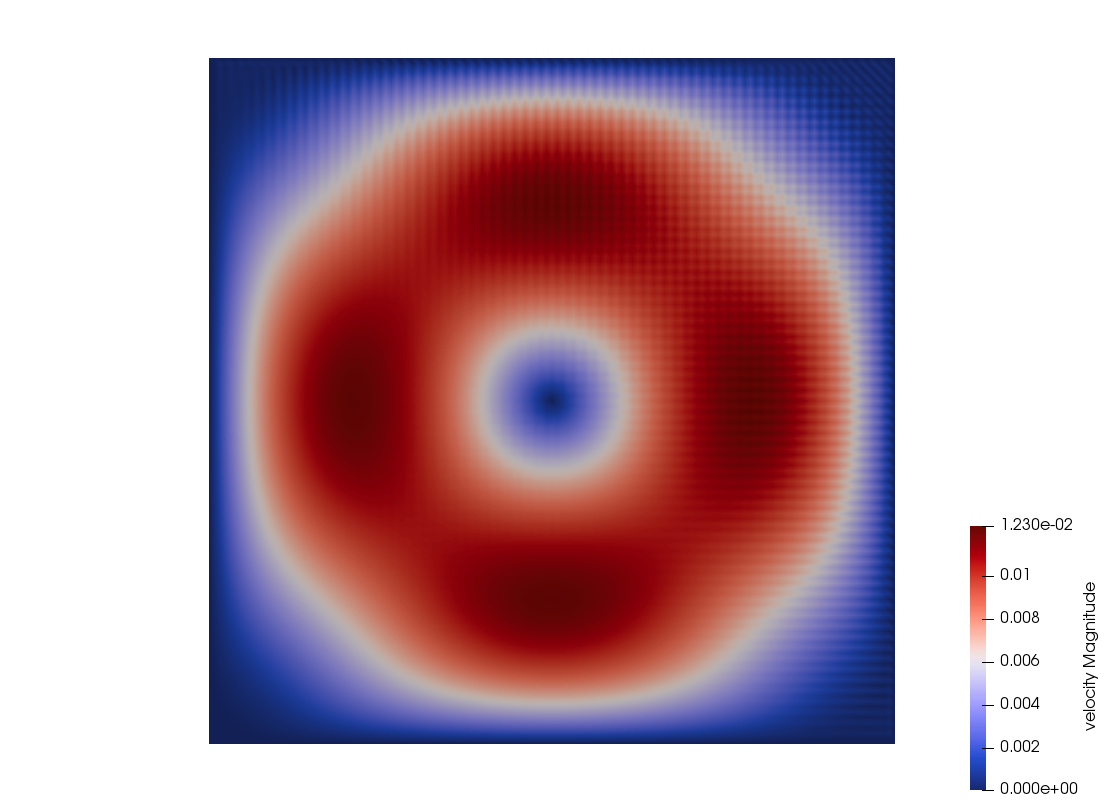
\includegraphics[width=3cm]{python_codes/fieldstone_107/results/mms/q2q1/vel64}
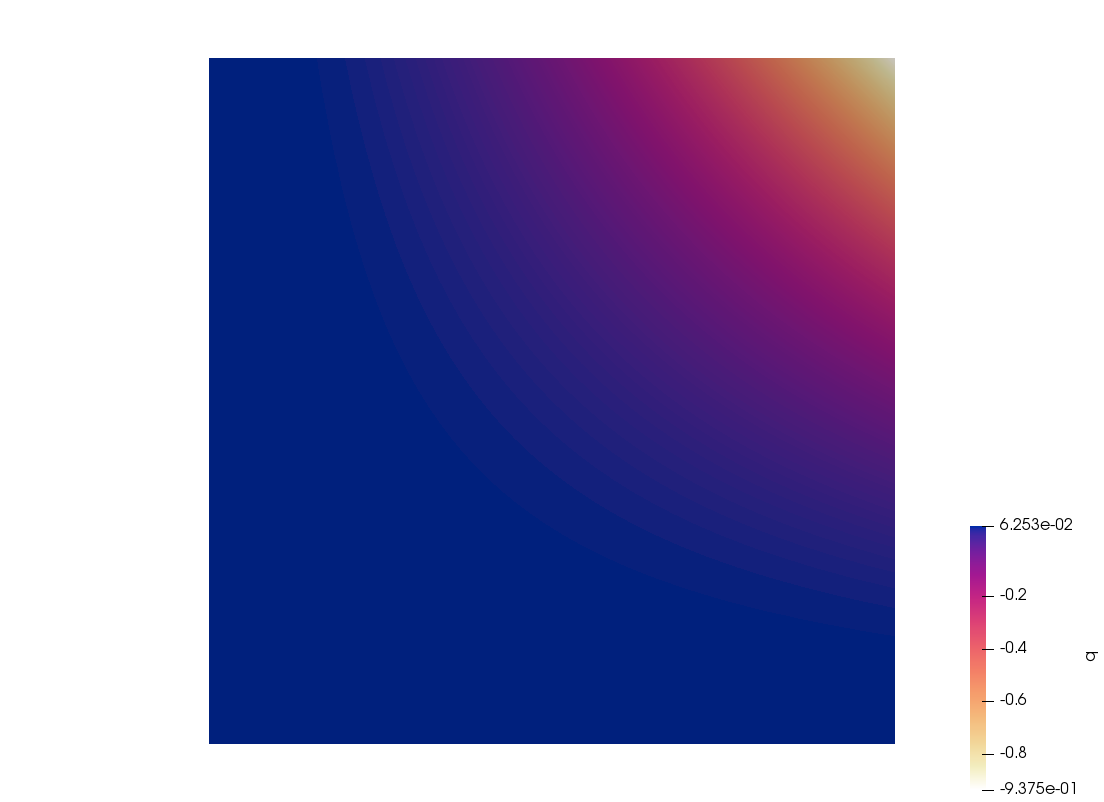
\includegraphics[width=3cm]{python_codes/fieldstone_107/results/mms/q2q1/q64}\\
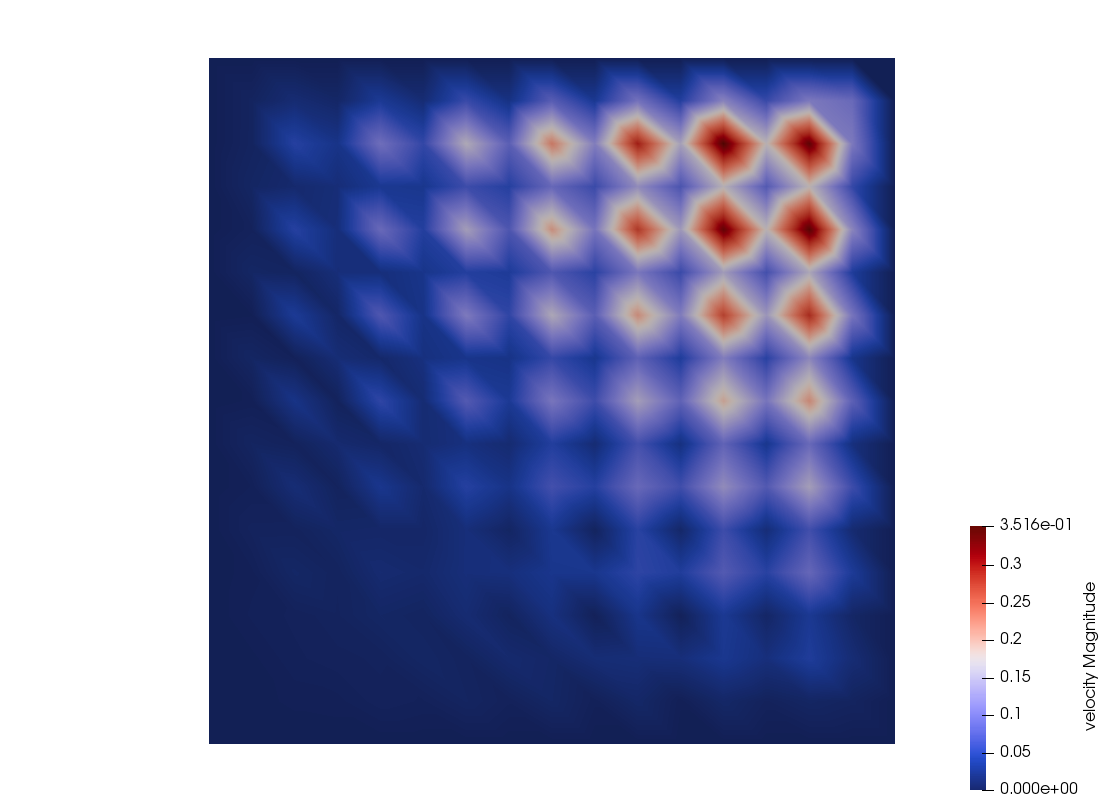
\includegraphics[width=3cm]{python_codes/fieldstone_107/results/mms/q2p1/vel08}
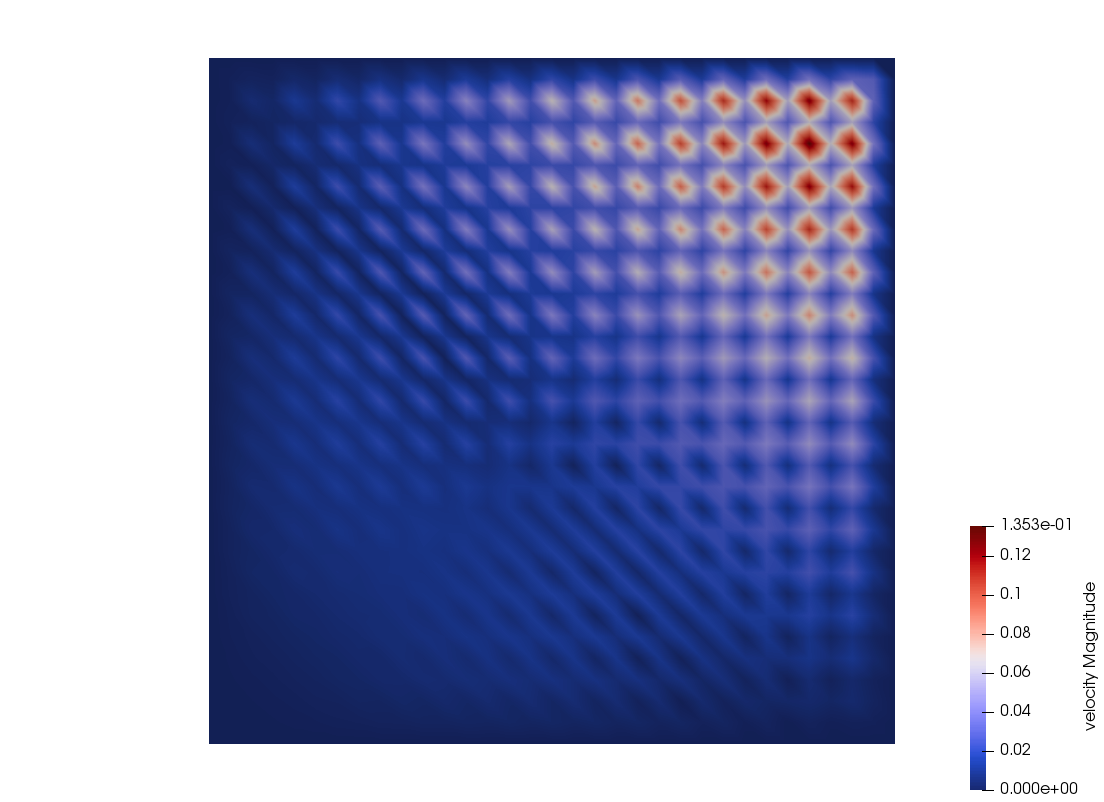
\includegraphics[width=3cm]{python_codes/fieldstone_107/results/mms/q2p1/vel16}
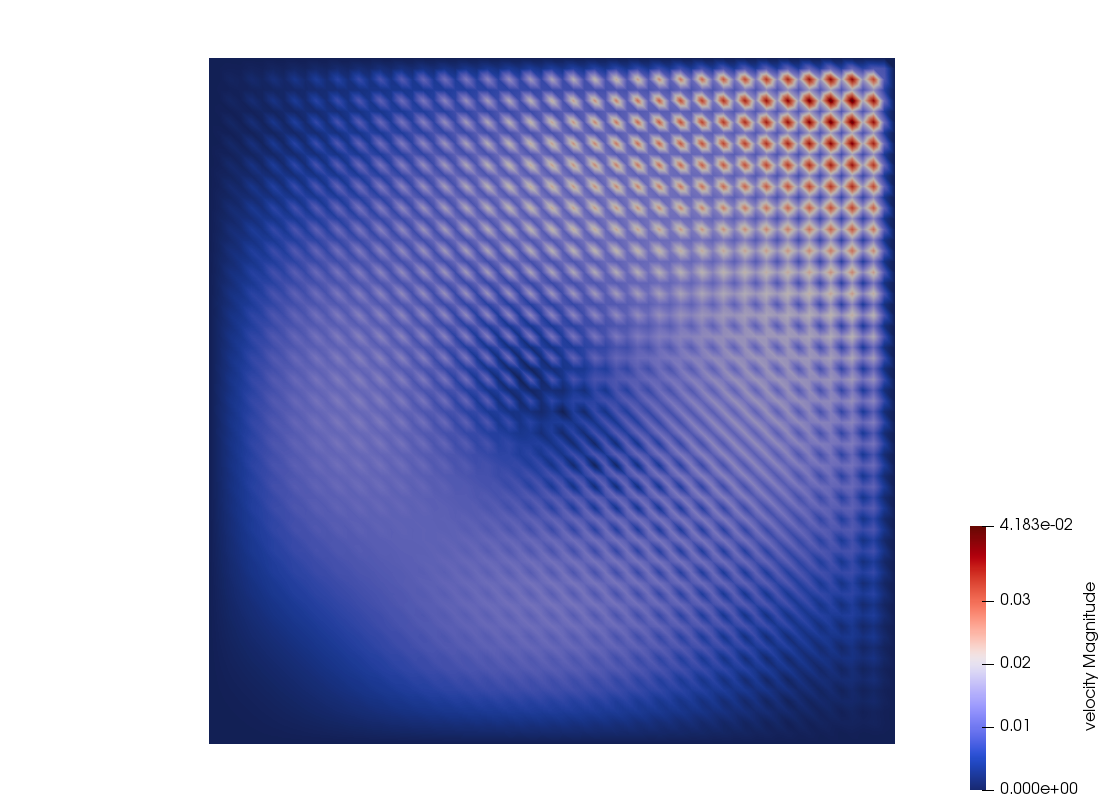
\includegraphics[width=3cm]{python_codes/fieldstone_107/results/mms/q2p1/vel32}
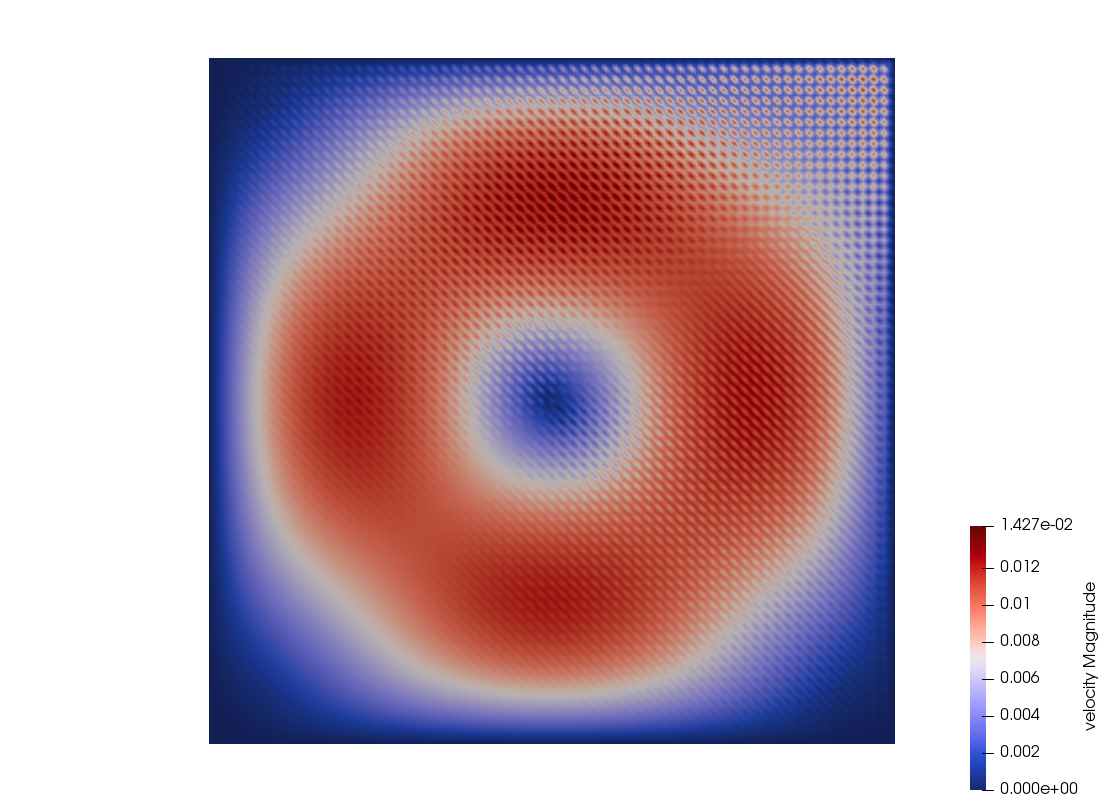
\includegraphics[width=3cm]{python_codes/fieldstone_107/results/mms/q2p1/vel64}
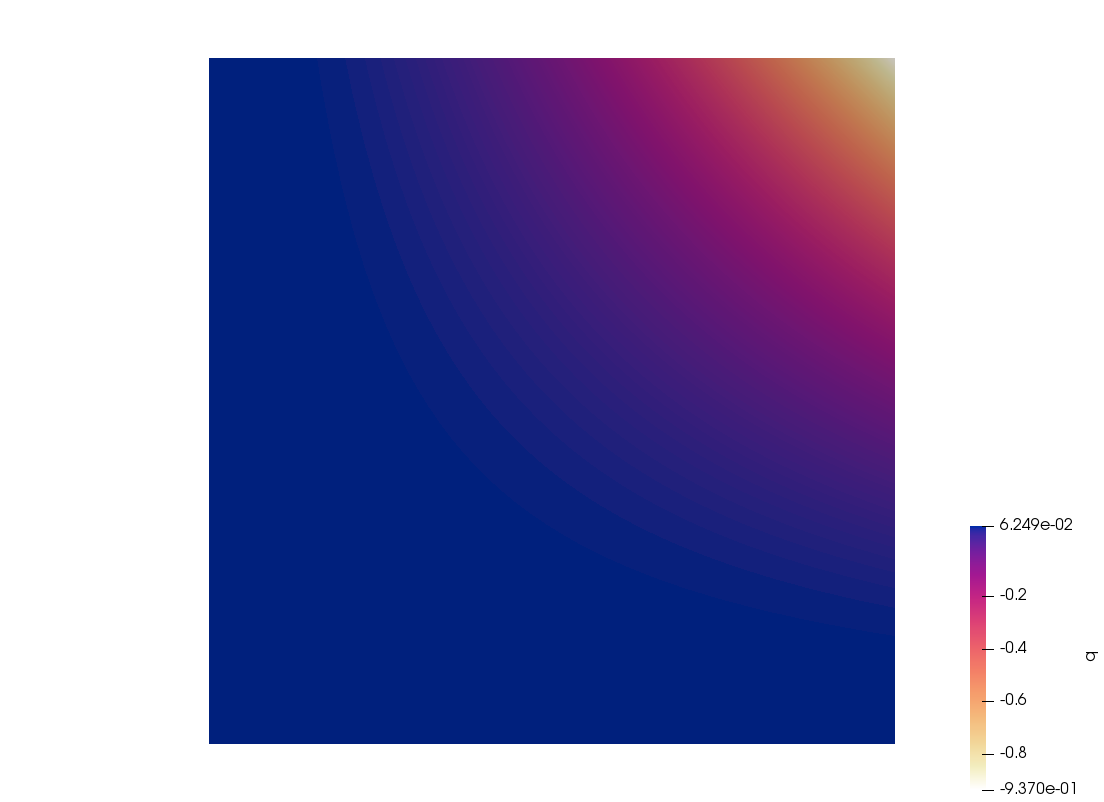
\includegraphics[width=3cm]{python_codes/fieldstone_107/results/mms/q2p1/q64}\\
{\captionfont Top row: $Q_2\times Q_1$, bottom row: $Q_2\times P_1$. From left to right, 8x8,
16x16, 32x32, 64x64. }
\end{center}

\begin{center}
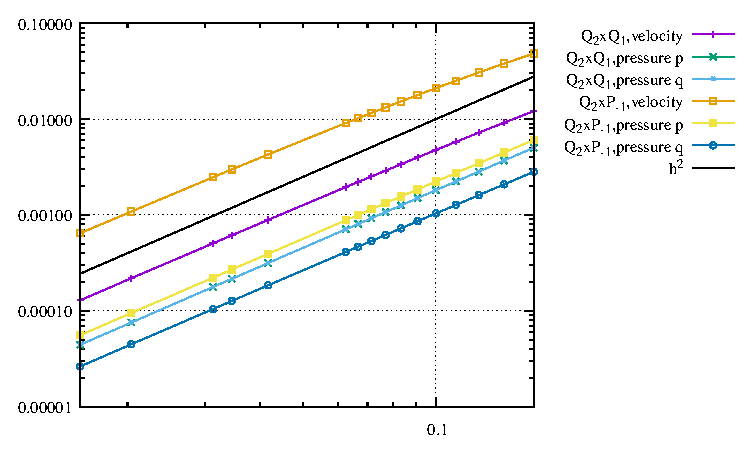
\includegraphics[width=8cm]{python_codes/fieldstone_107/results/mms/errors.pdf}\\
{\captionfont Velocity and pressure errors converge quadratically, which is quite
surprising...(?), for both elements $Q_2\times Q_1$ and $Q_2\times P_1$.}
\end{center}

{\color{orange} There is a big problem!! Even at 64x64 resolution the velocity artefacts 
are visible. I have checked and re-checked the mesh, connectivity, basis functions, 
derivatives, jacobian values, etc ... I have checked the elemental matrices against those of 
\stone~48. I am not sure what the problem is. Is this a conceptual
problem with the boundary conditions? }



%...............................................
\subsection*{Benchmark}

NOT FINISHED. See Palm \etal 1972. 

The solution can be expanded in a power series in the parameter $\xi$ defined by 
\[
\xi^2 = \frac{\Ranb-\Ranb_c}{\Ranb}
\qquad
\text{or,}\qquad
\Ranb = \frac{\Ranb_c}{1-\xi^2}
\]
The solution is then expected to follow:
\begin{eqnarray}
v &=& \xi v^{(1)} + \xi^2 v^{(2)} + \dots + \xi^n v^{(n)} + \dots \\
\theta &=& \xi \uptheta^{(1)} + \xi^2 \uptheta^{(2)} + \dots + \xi^n \uptheta^{(n)} + \dots 
\end{eqnarray}


\[
\Ranb_c = \frac{(\pi^2+a^2)^2}{a^2}
\]

\begin{eqnarray}
A_1&=&4\pi \left( \frac{\Ranb_{c,s}}{\Ranb_c} \right)^{1/2} \nonumber\\
A_2 &=& 0 \nonumber\\
A_3&=&2\pi \left(\frac{\Ranb_{c,s}}{\Ranb_c} \right)^{1/2} \left(1 + \frac{7}{24} \frac{\Ranb_{c,s}}{\Ranb_c}   \right) \nonumber\\
A_2 &=& 0 \nonumber\\
A_5&=&\frac{3\pi}{2} \left(\frac{\Ranb_{c,s}}{\Ranb_c} \right)^{1/2}
\left(1+\frac{7}{12} \frac{\Ranb_{c,s}}{\Ranb_c} -
\frac{173}{3\cdot24\cdot24} \left(\frac{R_{0s}}{R_0}\right) ^2 
\right) \nonumber\\
A_6 &=& 0 \nonumber
\end{eqnarray}


\[
\Nunb
\simeq 1 + 2 \frac{\Ranb_{c,s}}{\Ranb_c} \eta^2
+ 2 \frac{\Ranb_{c,s}}{\Ranb_c}
\left( 1 -\frac{17}{24}\frac{\Ranb_{c,s}}{\Ranb_c} \right) \eta^4
+2 \frac{\Ranb_{c,s}}{\Ranb_c}
\left( 
1 -\frac{17}{12}\frac{\Ranb_{c,s}}{\Ranb_c}
+ \frac{191}{288} \left(\frac{\Ranb_{c,s}}{\Ranb_c}\right) ^2
\right) \eta^6 
\]



\begin{center}
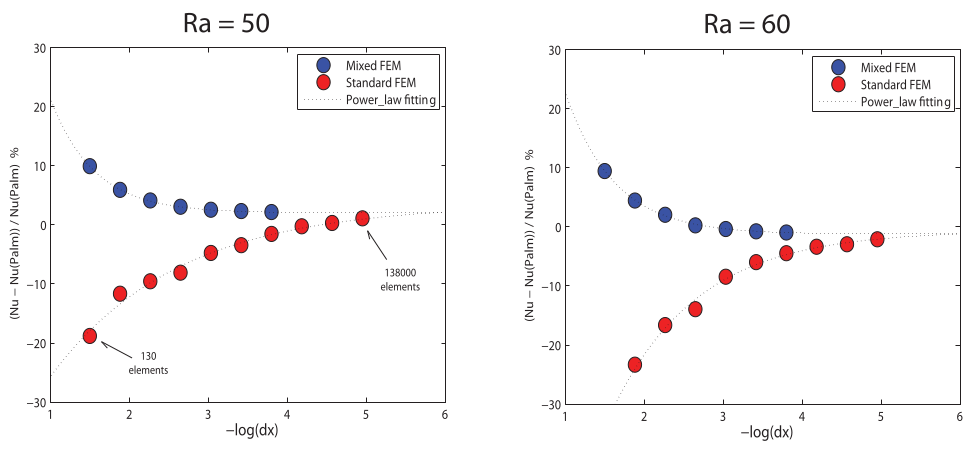
\includegraphics[width=14cm]{python_codes/fieldstone_107/images/souche_bench}\\
Taken from Souche, poster EGU, 2010. Standard FEM: $Q_2$ pressure, 
$Q_1$ temperature, $Q_1$ velocity. 
Mixed FEM: $P_{-1}$ pressure, $Q_2$ temperature, $Q_2$ velocity.
\end{center}





%...............................................
\subsection*{Onset and steady state of Darcy-B\'enard convection}

Let us consider a system heated from below and cooled from the top. We employ a 
grid consisting of $nelx\times nely$ elements and horizontal periodic boundary conditions are imposed. 
The temperature at the top $T_t$, is set to 100\si{\celsius}, while the temperature at the 
bottom of the domain is higher, $T_b$=110\si{\celsius}. The initial temperature field in the system is defined 
as a linear gradient between $T_b$ and $T_t$ with a randomness of 1\% to trigger the 
instabilities needed for convection to occur. 

\begin{center}
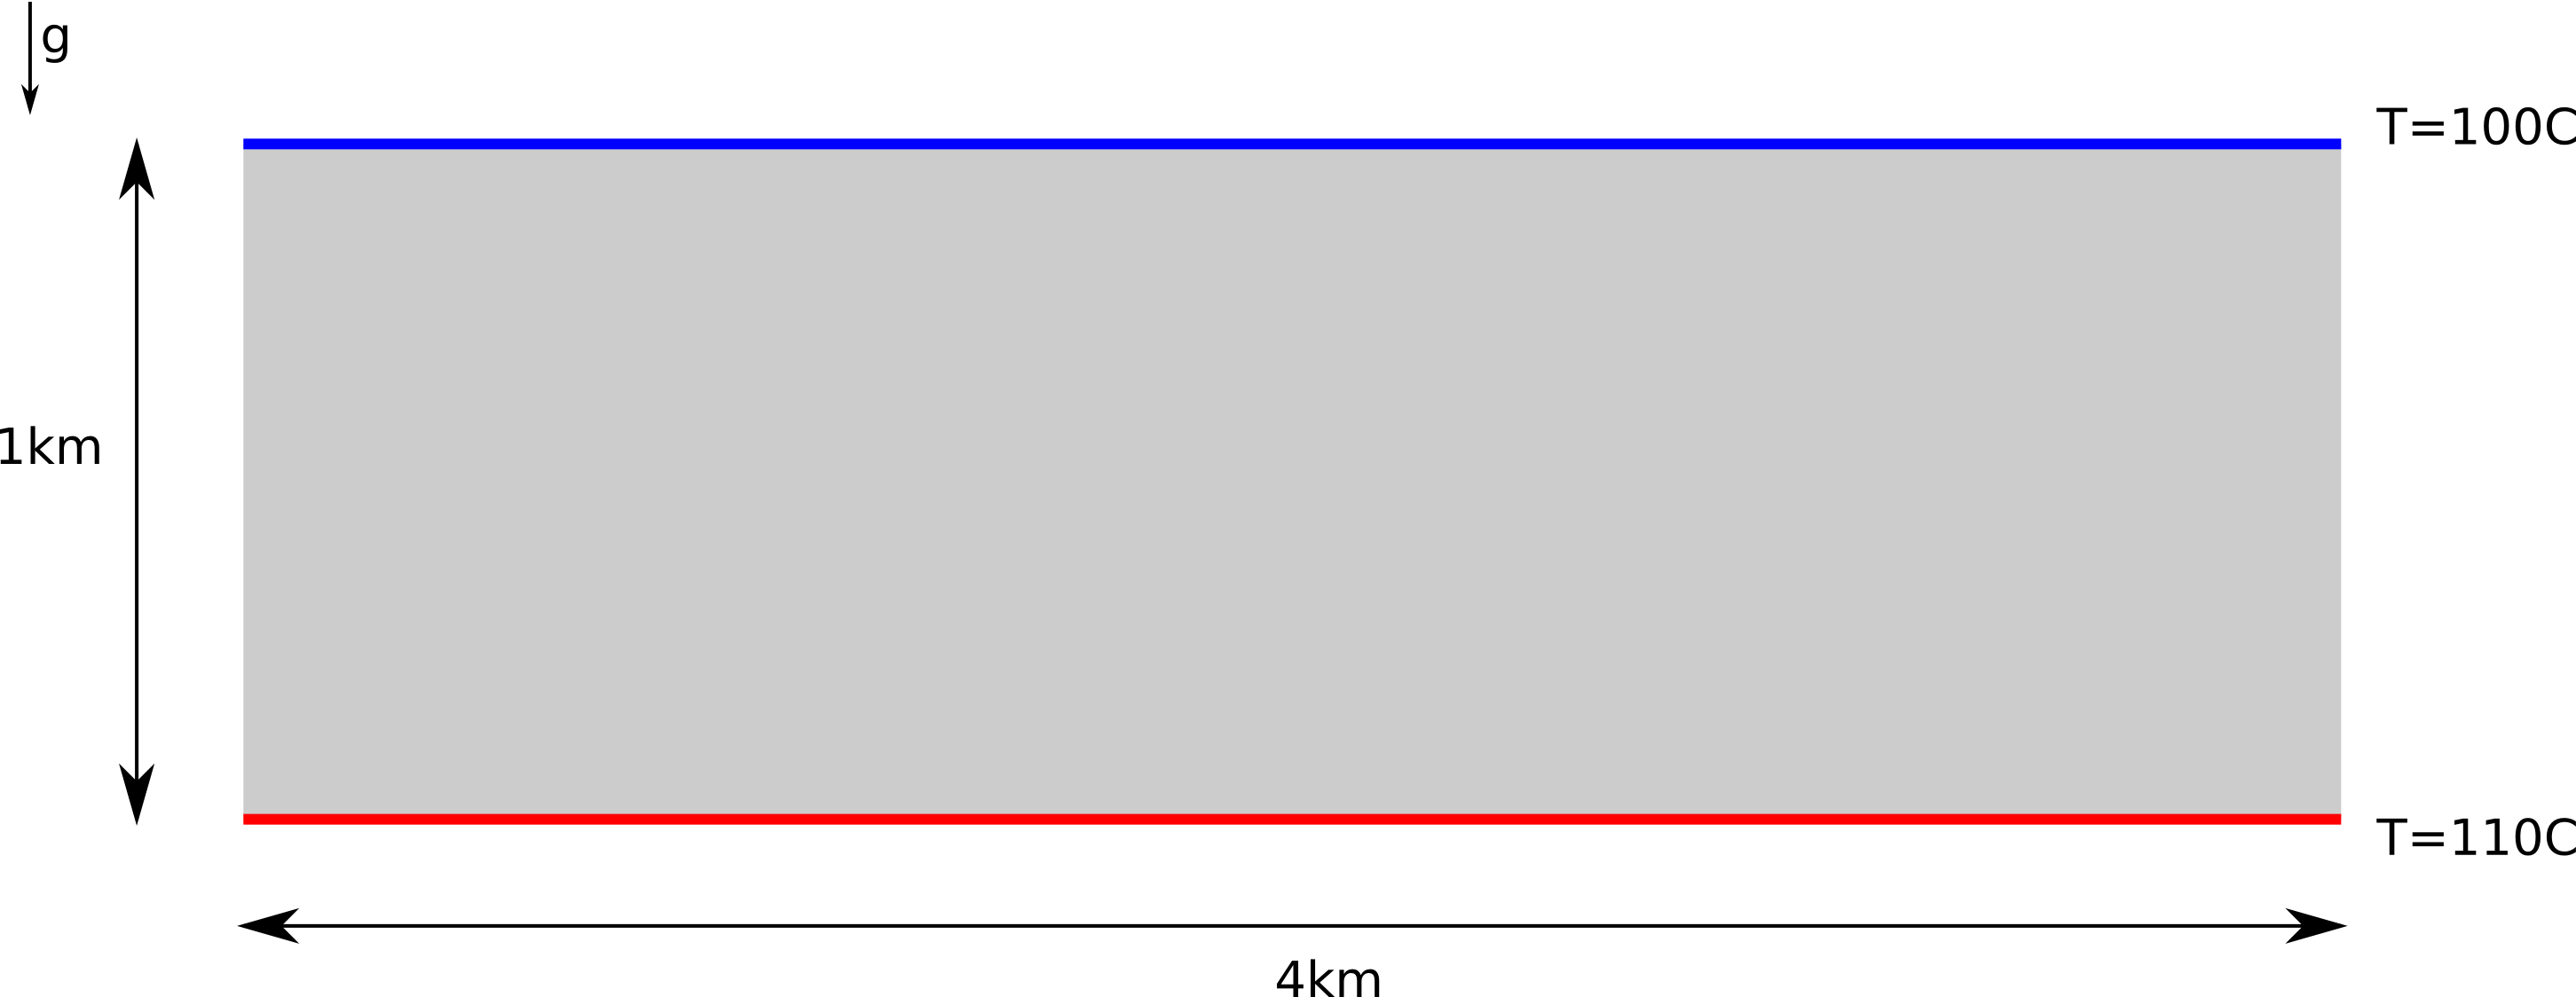
\includegraphics[width=7cm]{python_codes/fieldstone_107/images/drawing}\\
{\captionfont Setup for the experiment}
\end{center}

\begin{center}
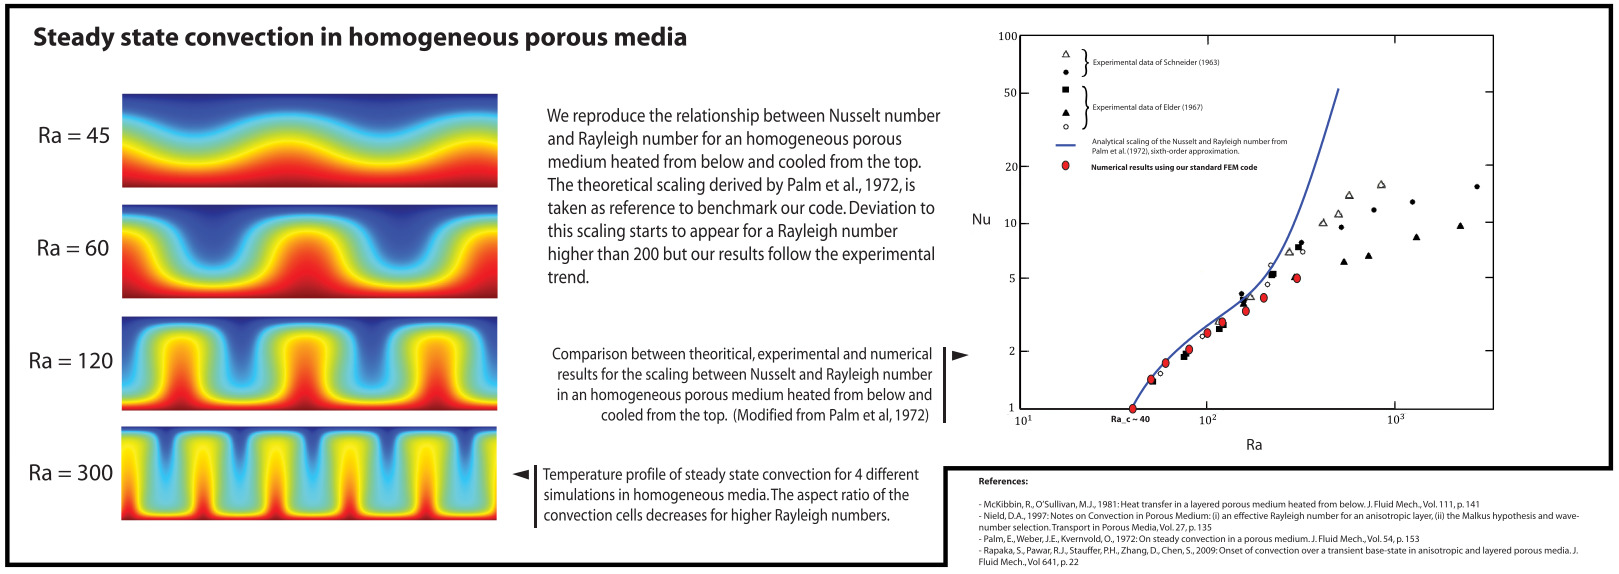
\includegraphics[width=14cm]{python_codes/fieldstone_107/images/souche_conv}
\end{center}

Only the value of the bottom temperature is varied to change the $\Ranb$ number value. 
All other material parameters are kept constant.
Below a critical $\Ranb$ number, the system is stable and no convection patterns develop. Heat 
is transported only by diffusion.
The heat flux is then given by $\vec{q}_{diff}=-k \vec{\nabla} T_f=-k (T_b-T_t)/L_y$.
Above a critical $\Ranb$ number, convection occurs in the system so that heat is transported 
both by advection and diffusion. 
One can measure $\vec{q}_T$ at the top of the simulation domain (averaged over the whole length) and 
the Nusselt number $\Nunb$ can be computed as follows:
\[
\Nunb=\frac{(Heat Flux)_{total}}{(Heat Flux)_{diff}} 
= \frac{\langle - k \vec{\nabla}T \cdot \vec{n}\rangle_{top}}{ -k (\Delta T)/L_y}
\]
Obviously for sub-critical Rayleigh flows, the Nusselt number is equal to 1. 

\begin{center}
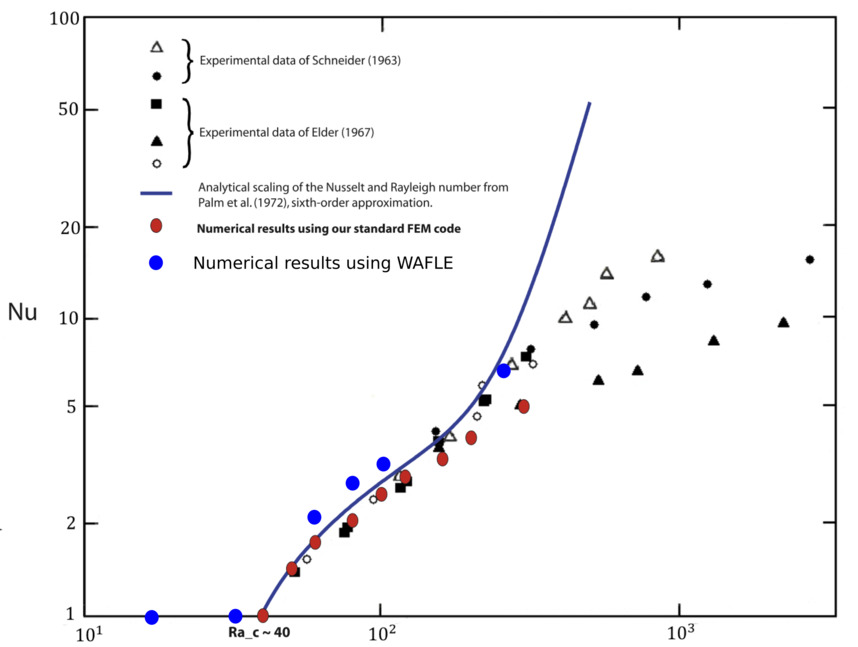
\includegraphics[width=9cm]{python_codes/fieldstone_107/images/NuRa2}\\
In WAFLE: $200 \times 50$ elements, horizontal periodic boundary conditions.\\ Domain is 4x1km. Permeability = 1e-12. porosity 0.99. 2 phases.  
\end{center}


\Literature: Banu \& Rees \cite{bare02}
